\documentclass[11pt]{article}
\usepackage[utf8]{inputenc}
\usepackage[T1]{fontenc}
\usepackage{lmodern}
\usepackage[margin=1in]{geometry}
\usepackage{amsmath,amssymb}
\usepackage{graphicx}
\usepackage{booktabs}
\usepackage{float}
\usepackage{xcolor}
\usepackage{enumitem}
\usepackage{tikz}
\usetikzlibrary{positioning,arrows.meta,calc}
\usepackage{xurl}
\usepackage{seqsplit}
\usepackage{hyperref}

\newcommand{\clip}[1]{\texttt{#1}}
\newcommand{\hash}[1]{\texttt{\seqsplit{#1}}}
\sloppy

\title{MaCVi@WACV 2027 Maritime Visual Odometry Challenge\\Factsheet}
\author{Vedran Mo\v{s}kov$^{1}$, Matej Fabijani\'c$^{2}$, Fausto Ferreira$^{2,1}$\\[4pt]
\parbox{0.9\textwidth}{\centering\normalsize
$^{1}$CoE MARBLE -- Centre of Excellence in Maritime Robotics and Technologies for Sustainable Blue Economy,
Zagreb, Croatia\\
$^{2}$University of Zagreb Faculty of Electrical Engineering and Computing, Zagreb, Croatia}}
\date{}

\begin{document}
\maketitle

\section{Team details}\label{sec:team}
\begin{itemize}
  \item \textbf{Team name (as on macvi.org):} UNIZG FER LABUST / MARBLE
  \item \textbf{Team leader name:} Vedran Mo\v{s}kov
  \item \textbf{Team leader institution and email:}\\
    CoE MARBLE -- Centre of Excellence in Maritime Robotics and Technologies for Sustainable Blue Economy, Zagreb, Croatia\\
    Email: \href{mailto:vedran.moskov@marble.eu}{vedran.moskov@marble.eu}
  \item \textbf{Team leader's macvi.org user ID:} 2078
  \item \textbf{Rest of the team members (name, macvi.org user ID):}
    \begin{itemize}
      \item[--] Matej Fabijani\'c (team owner on macvi.org), user ID 392
      \item[--] Fausto Ferreira, user ID 2079
    \end{itemize}
  \item \textbf{Affiliations:} CoE MARBLE -- Centre of Excellence in Maritime Robotics and Technologies for Sustainable Blue Economy, Zagreb, Croatia; University of Zagreb Faculty of Electrical Engineering and Computing, Zagreb, Croatia
  \item \textbf{Author list for the summary paper, in your team's author order} (full name, affiliation, e-mail, OpenReview profile ID):
    \begin{enumerate}
      \item Vedran Mo\v{s}kov, CoE MARBLE -- Centre of Excellence in Maritime Robotics and Technologies for Sustainable Blue Economy, \href{mailto:vedran.moskov@marble.eu}{vedran.moskov@marble.eu},
        \texttt{\textasciitilde Vedran\_Mo\v{s}kov1}
      \item Matej Fabijani\'c, University of Zagreb Faculty of Electrical Engineering and Computing, \href{mailto:matej.fabijanic@fer.hr}{matej.fabijanic@fer.hr},
        \texttt{\textasciitilde Matej\_Fabijani\'c1}
      \item Fausto Ferreira, University of Zagreb Faculty of Electrical Engineering and Computing and CoE MARBLE -- Centre of Excellence in Maritime Robotics and Technologies for Sustainable Blue Economy, \href{mailto:fausto.ferreira@fer.hr}{fausto.ferreira@fer.hr},
        \texttt{\textasciitilde Fausto\_Ferreira1}
    \end{enumerate}
  \item \textbf{Team website URL (if any):} none
  \item \textbf{Final entry (the upload selected as final entry in the dashboard):} submission ID 19444 (model name
    \texttt{med3-flow-pi3x-omega-ir}, 28~October~2026), uploaded by user ID 392, score shown on the leaderboard
    11.02\,\% (mean relative-position drift, \% of segment length)
  \item \textbf{Code repository and model weights:} \url{https://github.com/VMoskov/lookout-vo-challenge}, branch \texttt{fermarble-history},
    public, no expiry. The weights are the unmodified public checkpoints listed in
    Section~\ref{sec:repro}: \texttt{dpvo.pth} comes from the DPVO authors' \texttt{models.zip}, Pi3X, VGGT-1B
    and PanSR are downloaded from Hugging Face by the code, and VGGT-$\Omega$ requires gated access
    (\url{https://huggingface.co/facebook/VGGT-Omega}): the organizers need to request access there.
  \item \textbf{Artifact traceability:} Tag \texttt{final-entry} (\texttt{7fa87f3}): final configuration; rebuilding from it
    with the cached model outputs reproduces the submitted bundle bit-exactly. Later commits add run scripts,
    environment lock files, the cached model outputs, documentation and this factsheet. Final artifact file name
    \path{runs/submission_test_pi3x_ir_kwide_crop_ens_w32mean_vwwide_sf-hsnear_omega512-vis_wmean_ir-omega.json};
    SHA-256 of the final artifact
    \hash{f5e361160dd1dedad0b22de25e7e0175661bc129a2ffcb00724547e4ac4e9a27}, produced on x86\_64 (AMD Ryzen~9 7900)
    with an NVIDIA GeForce RTX 4070 Ti SUPER
\end{itemize}

\section{Global method description}\label{sec:method}

\begin{figure}[h]
  \centering
  \resizebox{\linewidth}{!}{% Overview of the final entry (med3-flow-pi3x-omega-ir); \input by main.tex.
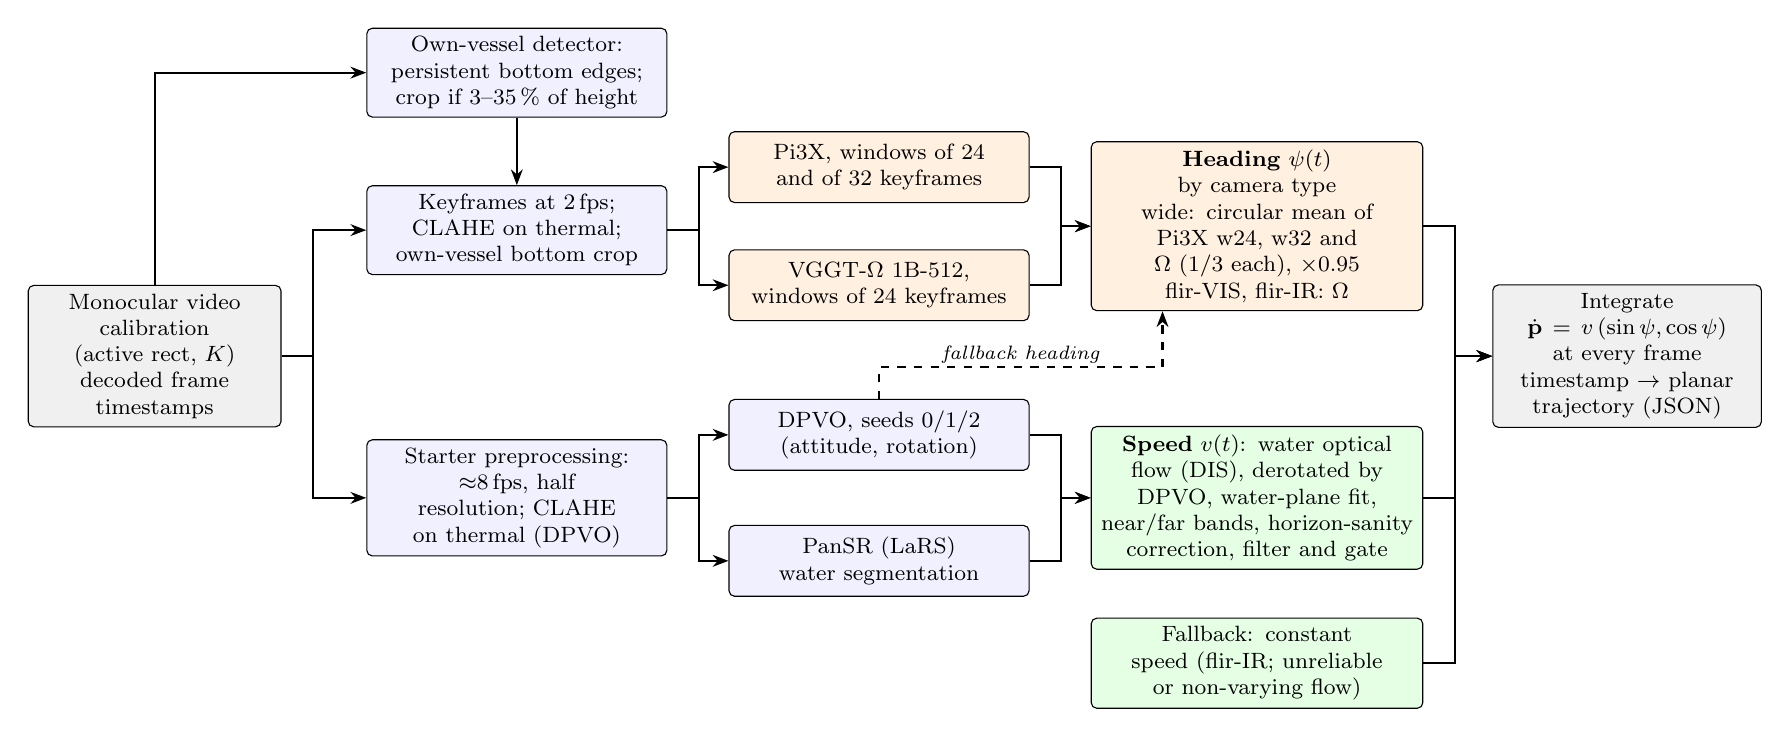
\begin{tikzpicture}[
    font=\footnotesize,
    box/.style={draw, rounded corners=2pt, align=center, inner sep=3pt, minimum height=9mm,
                text width=#1, execute at begin node=\hyphenpenalty 10000\relax},
    box/.default=36mm,
    io/.style={box=#1, fill=gray!12}, io/.default=30mm,
    pre/.style={box=#1, fill=blue!6}, pre/.default=36mm,
    head/.style={box=#1, fill=orange!12}, head/.default=36mm,
    spd/.style={box=#1, fill=green!10}, spd/.default=40mm,
    arr/.style={-{Stealth[length=2mm]}, thick},
    lab/.style={font=\scriptsize\itshape, align=center, fill=white, inner sep=1pt}]

  % column 0: inputs
  \node[io] (in) at (0,0) {Monocular video\\calibration (active rect, $K$)\\decoded frame timestamps};

  % column 1: preprocessing
  \node[pre] (crop) at (4.6,3.6) {Own-vessel detector: persistent bottom edges; crop if 3--35\,\% of height};
  \node[pre] (kf)   at (4.6,1.6) {Keyframes at 2\,fps; CLAHE on thermal; own-vessel bottom crop};
  \node[pre] (pp)   at (4.6,-1.8) {Starter preprocessing: $\approx$8\,fps, half resolution; CLAHE on thermal (DPVO)};

  % column 2: models
  \node[head] (pi)  at (9.2,2.4) {Pi3X, windows of 24 and of 32 keyframes};
  \node[head] (om)  at (9.2,0.9) {VGGT-$\Omega$ 1B-512, windows of 24 keyframes};
  \node[pre]  (dp)  at (9.2,-1.0) {DPVO, seeds 0/1/2 (attitude, rotation)};
  \node[pre]  (seg) at (9.2,-2.6) {PanSR (LaRS) water segmentation};

  % column 3: heading and speed
  \node[head=40mm] (hf) at (14.0,1.65) {\textbf{Heading} $\psi(t)$ by camera type\\wide: circular mean of Pi3X w24, w32 and $\Omega$ (1/3 each), $\times0.95$\\flir-VIS, flir-IR: $\Omega$};
  \node[spd] (fl) at (14.0,-1.8) {\textbf{Speed} $v(t)$: water optical flow (DIS), derotated by DPVO, water-plane fit, near/far bands, horizon-sanity correction, filter and gate};
  \node[spd] (cs) at (14.0,-3.9) {Fallback: constant speed (flir-IR; unreliable or non-varying flow)};

  % column 4: integration
  \node[io=32mm] (int) at (18.7,0) {Integrate $\dot{\mathbf p}=v\,(\sin\psi,\cos\psi)$ at every frame timestamp $\rightarrow$ planar trajectory (JSON)};

  % arrows
  \draw[arr] (in.north) |- (crop.west);
  \draw[arr] (in.east) -- ++(4mm,0) |- (kf.west);
  \draw[arr] (in.east) -- ++(4mm,0) |- (pp.west);
  \draw[arr] (crop.south) -- (kf.north);
  \draw[arr] (kf.east) -- ++(4mm,0) |- (pi.west);
  \draw[arr] (kf.east) -- ++(4mm,0) |- (om.west);
  \draw[arr] (pp.east) -- ++(4mm,0) |- (dp.west);
  \draw[arr] (pp.east) -- ++(4mm,0) |- (seg.west);
  \draw[arr] (pi.east) -- ++(4mm,0) |- (hf.west);
  \draw[arr] (om.east) -- ++(4mm,0) |- (hf.west);
  \draw[arr] (dp.east) -- ++(4mm,0) |- (fl.west);
  \draw[arr] (seg.east) -- ++(4mm,0) |- (fl.west);
  \draw[arr, dashed] (dp.north) -- ++(0,4mm) -| node[lab, pos=0.25, above] {fallback heading} ([xshift=-12mm]hf.south);
  \draw[arr] (hf.east) -- ++(4mm,0) |- (int.west);
  \draw[arr] (fl.east) -- ++(4mm,0) |- (int.west);
  \draw[arr] (cs.east) -- ++(4mm,0) |- (int.west);
\end{tikzpicture}
}
  \caption{Overview of the proposed method. Heading and speed are estimated separately and integrated into a
    planar trajectory at every released frame timestamp. Heading comes from pretrained multi-view geometry models
    (Pi3X and VGGT-$\Omega$) run on keyframes with the own vessel cropped away; speed comes from optical flow on
    the water surface, derotated with DPVO's camera rotation, and falls back to a constant speed where the flow
    is unreliable. DPVO also provides the fallback heading.}
  \label{fig:overview}
\end{figure}

\paragraph{Overview.}
The metric aligns each predicted trajectory to the planar reference with one global Sim(3) and scores drift
over 100--800\,m segments, so only the shape of the path matters, not its scale or orientation. We therefore
predict a planar path from two separately estimated signals, the heading $\psi(t)$ and a relative speed
$v(t)$ (clip median $=1$), and integrate them with the trapezoid rule at every released frame timestamp $t_k$:
\begin{equation}
  \mathbf p_{k+1} = \mathbf p_k + \tfrac12\bigl(v_k\,\mathbf u(\psi_k) + v_{k+1}\,\mathbf u(\psi_{k+1})\bigr)(t_{k+1}-t_k),
  \qquad \mathbf u(\psi) = (\sin\psi, \cos\psi, 0).
\end{equation}
The decoded frame timestamps are used for all time integration and for all temporal resampling; the camera
calibration (active image rectangle and intrinsics, as released) is used by the starter preprocessing, by the
heading definition and by the water-plane geometry of the speed estimate. No other input is used.

\paragraph{Heading.}
For a run of camera-to-world rotations $R_i$ (DPVO poses, or per-window rotations of a multi-view model chained
across overlapping windows), the up direction is estimated as $\mathbf n=-\overline{R_i\mathbf e_y}$ (minus the
mean camera $y$ axis), and the heading is the azimuth of the camera forward axis $R_i\mathbf e_z$ in the plane
perpendicular to $\mathbf n$, measured from the mean forward direction of the first 3\,s and unwrapped. Each
heading series is Gaussian-smoothed in time ($\sigma=1$\,s, on a 10\,Hz grid) and interpolated to every frame
timestamp. Heading sources:
\begin{itemize}[nosep]
  \item Pi3X~\cite{wang2025pi3,pi3x2025} on keyframes at 2\,fps, windows of 24 keyframes (overlap 4), and a second
    run with windows of 32;
  \item VGGT-$\Omega$ 1B-512~\cite{wang2026vggtomega} on the same keyframes, windows of 24 (overlap 4);
  \item VGGT-1B~\cite{wang2025vggt} is also run and passed to the fusion, but with weight 0 on every camera type,
    so it does not affect the final entry;
  \item DPVO~\cite{teed2023deep} (pinned commit \texttt{859bbbf}, through the starter's \texttt{track()} at 8\,fps)
    with seeds 0, 1, 2, combined by the per-frame circular median (``med3'').
\end{itemize}
Fusion by camera type, with the circular mean
$\bar\psi=\psi_1+\arg\sum_j w_j e^{\,i(\psi_j-\psi_1)}$:
\begin{itemize}[nosep]
  \item \textbf{wide:} Pi3X w24, Pi3X w32 and VGGT-$\Omega$ with weights $1/3$ each; the heading change since the
    start is multiplied by a yaw scale of 0.95 (fitted on train);
  \item \textbf{flir-VIS:} VGGT-$\Omega$ alone;
  \item \textbf{flir-IR:} VGGT-$\Omega$ alone (implemented as the agreement rule of \texttt{make\_predictions.py}
    with both members set to VGGT-$\Omega$ and both thresholds at $10^9$, so it applies whenever DPVO yields a heading).
\end{itemize}
Fallbacks: if no foundation-model run is usable for a clip, the DPVO 3-seed median heading is used; if no DPVO
run is usable either, a straight line. On the 20 test clips no fallback heading was needed: every clip uses the
foundation-model heading above.

\paragraph{Speed.}
Relative speed comes from dense optical flow (OpenCV DIS~\cite{kroeger2016dis}, MEDIUM preset) between consecutive
$\approx$8\,fps frames (the frames DPVO sees) on wide and flir-VIS clips:
\begin{enumerate}[nosep]
  \item Water region: PanSR~\cite{zust2026pansr} water mask (every second 8\,fps frame) below the horizon, at least
    $1.5^\circ$ below it; pixels that never move (own hull, overlays) are removed.
  \item Horizon: from DPVO's per-frame attitude (seed 0) plus a mount correction (pitch, roll) fitted to the
    strongest horizontal edge along the predicted horizon, refitted in 20\,s windows.
  \item Water-plane model: a water pixel with ray $\mathbf r$ lies at $\mathbf X=\mathbf r/s\cdot h$ with
    $s=-\mathbf n_c\!\cdot\mathbf r$; between frames $i$ and $j$ the camera rotates by DPVO's $R_{ji}$ (rotation
    removed exactly) and translates by a horizontal $\mathbf c$ (in units of the unknown camera height $h$). The
    two unknowns of $\mathbf c$ are fitted to the flow by Huber-weighted Gauss--Newton; speed $=|\mathbf c|/\Delta t$,
    separately for a near and a far band of water pixels.
  \item Horizon-sanity correction (``hs''): in each 20\,s window where DPVO's horizon lies more than 20\,px below
    the segmented water edge, or crosses non-water pixels below it in more than 15\,\% of the columns, the flow
    pairs computed with the segmentation horizon (shift 0\,px) replace those of the DPVO horizon.
  \item Filter: bands normalised by their clip medians; a pair is reliable if $|\log(\text{near}/\text{far})|\le0.6$
    and then gets their geometric mean; disagreeing pairs get $\text{near}^{0.6}\text{far}^{0.4}$ (``near'' preference,
    not counted as reliable); 8\,s rolling median, clamped below at $0.25\times$ the clip median, gaps filled with the
    median.
  \item Fallback to constant speed for the whole clip if fewer than 80\,\% of the pairs are reliable, or if the
    coefficient of variation of the resulting profile is below 0.35 (flow is used only where speed really varies).
    flir-IR clips always use constant speed.
\end{enumerate}

\paragraph{Own-vessel crop.}
A ground-truth-free detector (\texttt{fermarble/jobs/static\_regions.py}) samples 60 frames per clip, keeps Canny
edges present at the same pixel in $\ge85\,\%$ of them, and takes the connected components that reach the bottom rows
(excluding tall thin masts, components in the outer 15\,\% of the width, i.e.\ HUD elements, and specks). The crop
fraction is the height of this block relative to the image height, capped at 50\,\%. Clips with a crop fraction of
3--35\,\% of the frame height (inclusive), on all camera types, have that fraction removed from the bottom of the
keyframes of Pi3X (both runs) and VGGT-$\Omega$ (\texttt{fermarble/jobs/select\_crops.py}). The lower bound is the
detector's own minimum block size; the upper bound was set by hand: detections at or near the detector's 50\,\% cap
are not used, since the true extent is unknown and cropping half the frame would remove most of the usable scene.
During development, the selection was restricted to wide and flir-VIS cameras, with the one flir-IR test clip added
manually; the released code applies the rule to all cameras and yields identical crops on all 20 test clips.
Cropped test clips: 093 (20.6\,\%), 094 (10.0), 095 (8.9), 096 (16.7), 098 (4.4), 099 (16.1), 100 (5.6), 104 (35.0),
105 (9.4), 108 (28.9), 109 (23.3), 111 (15.6). DPVO, segmentation and flow use uncropped frames.

\paragraph{Thermal.}
On flir-IR clips, CLAHE~\cite{zuiderveld1994clahe} (clip limit 2.0, $8\times8$ tiles) is applied to the frames
DPVO sees and to the keyframes of the multi-view models.

\paragraph{What is new.}
See ``Novelty degree'' below. All models are used with their published pretrained weights and no fine-tuning in the final entry.

\begin{itemize}
  \item \textbf{Pretrained or external methods / models used (at any stage, if any):}
    \begin{itemize}[nosep]
      \item DPVO~\cite{teed2023deep}, code \url{https://github.com/princeton-vl/DPVO} commit \texttt{859bbbf}, checkpoint
        \texttt{dpvo.pth} (from the authors' \texttt{models.zip}); pretrained on TartanAir~\cite{wang2020tartanair}.
      \item Pi3X~\cite{pi3x2025}, checkpoint \texttt{yyfz233/Pi3X} \texttt{model.safetensors} (Hugging Face revision
        \texttt{bb1deea}), weights CC BY-NC 4.0. Pi3X has no separate paper; it is described as an upgrade of
        $\pi^3$~\cite{wang2025pi3}, which was trained on 15 datasets (GTA-SfM, CO3D, WildRGB-D, Habitat, ARKitScenes,
        TartanAir, ScanNet, ScanNet++, BlendedMVG, MatrixCity, MegaDepth, Hypersim, Taskonomy, Mid-Air and an
        internal dynamic-scene dataset) with encoder and alternating-attention weights initialised from VGGT.
        Pi3X's own training data: not documented by the authors.
      \item VGGT-$\Omega$ 1B-512~\cite{wang2026vggtomega}, checkpoint \texttt{facebook/VGGT-Omega}
        \texttt{vggt\_omega\_1b\_512.pt} (official, gated), FAIR Noncommercial Research License; code
        \url{https://github.com/facebookresearch/vggt-omega} commit \texttt{48b23c8}. Per its paper: trained on public
        datasets including Aria, BEDLAM, BEHAVIOR-1K, Co3Dv2, DL3DV, Dynamic Replica, EDEN, EFM3D, HOT3D, Habitat,
        Hypersim, Mapfree, Mapillary Metropolis, MPSD, MegaDepth, MegaSynth, Mid-Air, MVS-Synth, ParallelDomain-4D,
        Replica, SAIL-VOS, the ScanNet series, TartanAirV2, TartanGround, Taskonomy, UnrealStereo4K, Virtual KITTI,
        Waymo and WildRGBD, plus internal datasets and internally annotated Internet videos; the vision transformer
        is initialised from DINOv3. Only the camera head is used (the dense head is not loaded).
      \item VGGT-1B~\cite{wang2025vggt}, checkpoint \texttt{facebook/VGGT-1B} \texttt{model.safetensors} (revision
        \texttt{860abec}, original non-commercial checkpoint); run, but with weight 0 in the final entry. Trained on
        Co3Dv2, BlendMVS, DL3DV, MegaDepth, Kubric, WildRGB, ScanNet, HyperSim, Mapillary, Habitat, Replica, MVS-Synth,
        PointOdyssey, Virtual KITTI, Aria Synthetic Environments, Aria Digital Twin and a synthetic dataset of
        artist-created assets.
      \item PanSR~\cite{zust2026pansr}, Swin-L model, checkpoint \texttt{lojzezust/pansr-lars-swinl}
        \texttt{model.safetensors} (revision \texttt{ee6ae6a}); code \url{https://github.com/lojzezust/PanSR} commit
        \texttt{148183f} (Apache-2.0), built on Detectron2~\cite{wu2019detectron2}; trained on
        LaRS~\cite{zust2023lars}. Backbone initialisation of the released checkpoint and weights licence: not documented
        by the authors (PanSR's README recommends the ImageNet-22k Swin-L backbone for training from scratch; the code is
        Apache-2.0).
    \end{itemize}
  \item \textbf{Additional data used in addition to the provided training split (at any stage, if any):} None in the
    final entry. One discarded experiment fine-tuned DPVO on an in-house MARBLE maritime dataset (camera, LiDAR and IMU); it was uploaded once (\#18848, 25.50\,\%) and is not part of the final entry.
  \item \textbf{Training description:} No training or fine-tuning in the final entry; all networks use the pretrained
    weights above. One discarded experiment fine-tuned DPVO on an in-house MARBLE maritime dataset (camera, LiDAR and IMU); it was uploaded once (\#18848, 25.50\,\%) and is not part of the final entry.
    The following constants were fitted against ground truth on the \emph{train} split only (\texttt{fermarble/oracle.py},
    the only code that reads references), by grid search minimising the mean drift of the official metric:
    \begin{itemize}[nosep]
      \item flow speed filter (\path{runs/speed-tune3/params_v3a_no_hjump.json}): band agreement tolerance 0.6,
        rolling window 8\,s, lower clamp 0.25, minimum reliable fraction 0.8, gate statistic CV with threshold 0.35;
      \item speed fix ``hs+near'' (\path{runs/speedfix/tune-vwwide/speedfix_best.json}): PanSR-masked flow, horizon
        shift 0\,px, window rule 20\,px below / 15\,\% crossing, near-band weight 0.6, near-only pairs not counted as reliable;
      \item wide yaw scale 0.95 (sweep 0.70--1.30, \path{runs/yaw-scale/fit.json}).
    \end{itemize}
    All other constants (smoothing $\sigma$, keyframe rate, windows, fusion weights, crop bounds, flow geometry) are
    design choices or were selected between candidates on val (see ``How the development clips were used'').
  \item \textbf{Testing description:}
    \begin{itemize}[nosep]
      \item Input resolution and frame rate: DPVO, flow and segmentation use the starter preprocessing (active
        rectangle, half resolution, trimmed to multiples of 16): $528\times960$ for wide and flir-VIS,
        $528\times672$ for flir-IR, at $\approx$8\,fps (every 3rd frame of 25\,fps, every 4th of 30\,fps video).
        Pi3X and VGGT keyframes are resized to 518\,px wide and centre-cropped to a multiple of 14 rows
        ($280\times518$ for 16:9, $406\times518$ for flir-IR, before the own-vessel crop); VGGT-$\Omega$ keyframes to
        704\,px wide and a multiple of 16 rows ($384\times704$, $544\times704$); keyframes at 2\,fps. PanSR segments
        the $528$-row frames at native size, every second frame.
      \item Scale recovery: none; speed is relative within a clip and the metric's Sim(3) absorbs the scale.
      \item Tracking failures: on the test set the heading of every clip comes from the foundation models, so DPVO
        tracking failures (e.g.\ on 096, 100, 104, where DPVO barely moves) do not reach the heading; non-finite DPVO poses
        are dropped before computing headings, and the fallbacks above cover clips without usable runs. The flow uses
        DPVO seed 0 for rotation and horizon; where the flow is unreliable, the clip falls back to constant speed.
      \item Speed per test clip: flow speed on 092 (wide), 094 (flir-VIS), 103 (wide), 109 (flir-VIS); constant speed
        on 093, 095, 097, 099, 101, 105, 106, 107, 110, 111, 112 (flow too uniform: CV gate), on 096, 098, 104, 108
        (fewer than 80\,\% reliable pairs) and on 100 (flir-IR, constant by design). The horizon-sanity correction
        fires on 103 and 104.
      \item Smoothing: heading $\sigma=1$\,s; speed 8\,s rolling median. No other post-processing.
      \item Hardware: one NVIDIA GeForce RTX 4070 Ti SUPER (16\,GB), AMD Ryzen 9 7900 (24 threads), 61\,GiB RAM.
    \end{itemize}
  \item \textbf{How the development clips were used:} Train (68 clips: 46 wide, 8 flir-VIS, 7 sionyx, 4 flir-IR,
    2 zoom, 1 infrared) was used to fit the constants listed under ``Training description''. Val (24 clips: 21 wide,
    2 zoom, 1 flir-IR: 005 007 008 009 012 016 018 020 025 028 037 038 046 050 052 053 057 059 064 066 072 077 080 086)
    was used for model selection and gating: a variant was kept only if it was not worse than the current pipeline on
    both train and val, with one exception (the own-vessel crop, see below). Val choices include the speed-filter variant without the horizon-jump gate, the wide fusion
    (1/3 each rather than VGGT-$\Omega$ alone) and VGGT-$\Omega$ for flir-IR (decided mainly on val clip 046). There
    are no flir-VIS clips in val, so flir-VIS choices rest on the 8 train clips. Val clips 038 and 077 (and train clip
    021) were inspected while designing the flow method. Dev drift of the final configuration as submitted: train 10.56\,\%,
    val 10.62\,\% (mean). The released crop rule additionally crops dev clips 019, 040 (flir-IR), 032 (sionyx) and
    028 (zoom); these were not re-evaluated. On dev, the flow uses the DPVO seed with the most finite poses; on test, seed 0.
  \item \textbf{Compliance with the challenge rules:} Yes. Inference uses only the monocular video, the released
    camera calibration and the decoded frame timestamps (no GPS, IMU, AIS, speed, heading or other clip-specific
    navigation signals); no validation or test videos were used for training, including self-supervised training.
  \item \textbf{Were the released test frames used in any way for training, fine-tuning, adaptation or
    tuning of the method?} Yes, but not for training or adaptation: no network was trained or adapted, and all fitted
    parameters were fitted on train. The test frames were used as follows:
    \begin{enumerate}[label=(\roman*),nosep]
      \item the horizon correction originated from inspecting frames of clips where the optical-flow speed failed,
        including test clips;
      \item candidate speed-correction variants had to pass ground-truth-free plausibility checks on the test clips
        they changed;
      \item the crop's upper bound was set after inspecting detector outputs on all clips, test included;
      \item a cropped DPVO rerun was done on test clips where DPVO did not track (096, 100, 104); it did not restore
        tracking and is not used in the final entry.
    \end{enumerate}
    The own-vessel crop is the one exception to the train-and-val rule: it was slightly worse on val
    (11.41 $\rightarrow$ 11.54\,\%) and better on train (12.35 $\rightarrow$ 12.16\,\%), and was included in the
    uploads because Pi3X's heading agreed better with VGGT's on the cropped test clips (ground-truth-free); it was
    kept because of the leaderboard results of \#19153 and \#19213 (below).
  \item \textbf{Which settings (seed, frame rate, resolution, thresholds, fallback rules, \dots) were chosen
    using leaderboard scores?} Each was applied identically to every clip. Uploads in order, with the leaderboard
    drift:
    \begin{itemize}[nosep]
      \item \#18724 (15~Oct, \texttt{dpvo-heading-\dots}): DPVO heading (seed~0) with constant speed: 22.14\,\%
        $\Rightarrow$ speed was the largest error on dev, so the optical-flow speed and the 3-seed median heading were
        developed next.
      \item \#18758 (16~Oct, \texttt{med3-flow-horizon}): DPVO 3-seed median heading with flow speed on wide and
        flir-VIS: 17.94\,\% $\Rightarrow$ adopted.
      \item \#18848 (19~Oct, \texttt{dpvo\_clamp\_mf}): a separate experiment by a team member: DPVO fine-tuned on an
        in-house MARBLE maritime dataset (camera with LiDAR and IMU used for supervision during training only):
        25.50\,\%. It did not learn that dataset reliably and scored worse on the leaderboard, so it was not used.
      \item \#18905 (20~Oct, \texttt{med3-flow-focal}): focal length $\times2.0$ on the flir-VIS clips ($\times1.0$
        where every $\times2.0$ DPVO run lost tracking: 096, 104): 18.99\,\% $\Rightarrow$ the released intrinsics
        ($\times1.0$) are kept for every clip.
      \item \#19023 (22~Oct, \texttt{med3-flow-vggtswitch}): DPVO/VGGT heading switch (VGGT's heading when it diverges
        from DPVO's by $>54.25^\circ$ within 60\,s): 14.74\,\% $\Rightarrow$ adopted, later superseded by the next item.
      \item \#19072 (23~Oct, \texttt{med3-flow-pi3x}): Pi3X heading on all wide and flir-VIS clips, VGGT/Pi3X agreement
        rule on flir-IR: 12.56\,\% $\Rightarrow$ foundation-model heading always on.
      \item \#19153 (24~Oct, \texttt{med3-flow-pi3x-kcrop-seg}): Pi3X heading + wide yaw scale 0.95 + own-vessel crop +
        segmentation-based speed correction (PanSR-masked flow with segmentation horizon, re-fitted filter thresholds):
        12.88\,\%; \#19213 (25~Oct, \texttt{med3-flow-pi3x-kcrop}): the same without the segmentation-based speed
        correction: 11.85\,\% $\Rightarrow$ that speed correction was dropped.
      \item \#19311 (26~Oct, \texttt{med3-flow-pi3x-kcrop-inpa}): automatic inpainting of own-vessel structure for
        Pi3X: 11.98\,\% $\Rightarrow$ dropped.
      \item \#19373 (27~Oct, \texttt{med3-flow-pi3x-kcrop-w32-\dots}): on top of \#19213, the Pi3X heading as the
        circular mean of the window-24 and window-32 runs, with VGGT at weight 0.1 on wide clips: 11.76\,\%
        $\Rightarrow$ adopted as the base of the final entry, which keeps the window-24/32 averaging.
      \item \#19444 (28~Oct, \texttt{med3-flow-pi3x-omega-ir}), final entry: on top of \#19373, VGGT-$\Omega$ (in place
        of VGGT in the wide fusion, 1/3 each with the two Pi3X runs; flir-VIS heading; flir-IR heading) and the gated
        speed correction (hs+near): 11.02\,\%. These two were added together in one upload, so their individual test
        effects are unknown.
      \item The final entry was selected in the dashboard as the upload with the lowest leaderboard score.
    \end{itemize}
    The own-vessel crop was always uploaded together with the wide yaw scale 0.95: \#19153 added the
    segmentation-based speed correction to both, and \#19213 left it out to separate the effects. From 12.56\,\%
    (\#19072) to 12.88\,\% (\#19153) and 11.85\,\% (\#19213), the speed correction was dropped and the yaw scale and
    crop were kept; the crop's test effect on its own, apart from the yaw scale, is unknown.
  \item \textbf{Novelty degree of the solution and whether it has been previously published:} The solution
    combines existing pretrained models (DPVO, Pi3X, VGGT-$\Omega$, PanSR) without training. Our contributions are the
    decomposition of the trajectory into a heading from multi-view geometry models and a separately estimated relative
    speed; the optical-flow speed estimator on the water surface (water-plane model with rotation removed using DPVO,
    near/far band agreement, horizon-sanity correction, reliability gate with fallback to constant speed); and the
    own-vessel crop. It has not been published.
  \item \textbf{Other methods and baselines tested (even if results were not competitive):} Dev numbers are mean drift
    (train / val) with the official evaluator; test numbers are leaderboard drift.
    \begin{itemize}[nosep]
      \item Plain DPVO trajectory (starter baseline): 58\,\% (the baseline figure we started from; not re-measured on all dev clips).
      \item DPVO heading + constant speed: 19.88 / 25.03 (seed 0; 22.14 on test); 3-seed circular median: 19.77 / 23.75.
      \item Flow speed on wide and flir-VIS: 17.94 on test.
      \item DPVO/VGGT heading switch: 14.74 on test; Pi3X heading always on: 12.60 / 11.47 dev, 12.56 test.
      \item Focal length changes: $\times2.0$ on flir-VIS improved train flir-VIS (17.15 $\rightarrow$ 7.74, 3-seed median, heading
        + constant speed) but scored 18.99 vs 17.94 on test; flir-IR $\times0.5$ / $\times0.75$ worse than $\times1.0$ on train;
        a zoom-aware flir-VIS yaw scale was not used.
      \item PanSR masking / segmentation-based speed correction (masked flow with segmentation horizon): better on dev, 12.88
        on test vs 11.85 without; the gated variant (hs+near) is in the final entry (dev 11.07 / 11.16 vs 12.05 / 11.36 without).
      \item Inpainting of own-vessel structure for Pi3X: 11.98 on test vs 11.85 without.
      \item CLAHE variants: DPVO with CLAHE on flir-IR improved the dev flir-IR 3-seed median (10.8 $\rightarrow$ 8.0) but
        hurt the colour low-light ``infrared'' clip (42.9 $\rightarrow$ 52.4), so it is applied to flir-IR only; a 5-seed
        CLAHE DPVO median and Pi3X/VGGT without CLAHE gave no improvement on dev flir-IR.
      \item Also tested on dev and not used: DPVO \texttt{GRADIENT\_BIAS} patch selection (wide heading-only 9.25
        $\rightarrow$ 9.43), Pi3X/VGGT heading mean, heading-smoothing sweep (no effect), flow derotated with Pi3X
        rotation (val 18.07 vs 11.41), VGGT-$\Omega$ alone on wide (better train, worse val).
      \item DPVO fine-tuned on an in-house MARBLE maritime dataset (camera, with LiDAR and IMU for supervision during
        training only), a separate experiment by a team member: it did not learn that dataset reliably; 25.50 on test
        (\#18848); not used.
    \end{itemize}
\end{itemize}

\begin{table}[H]
  \centering
  \resizebox{\linewidth}{!}{%
  \begin{tabular}{ccccccc}
    \toprule
    Method & Input size & Frame rate & Pretrained & Extra data & \# Params. (M) & GPU\\
    \midrule
    \begin{tabular}[c]{@{}c@{}}med3-flow-pi3x-\\omega-ir\end{tabular}
      & \begin{tabular}[c]{@{}c@{}}DPVO/flow $528\times960$\\Pi3X $280\times518$\\$\Omega$ $384\times704$\end{tabular}
      & \begin{tabular}[c]{@{}c@{}}$\approx$8 (DPVO, flow)\\2 (Pi3X, $\Omega$)\end{tabular}
      & Yes & No
      & \begin{tabular}[c]{@{}c@{}}3.5 + 1360.0 + 1144.1\\+ 249.9 (+ 1256.5)\end{tabular}
      & \begin{tabular}[c]{@{}c@{}}RTX 4070 Ti\\SUPER 16\,GB\end{tabular}\\
    \bottomrule
  \end{tabular}}
  \caption{Summary of the method used for the final entry. Input sizes for 16:9 wide/flir-VIS video before the
    own-vessel crop (flir-IR: $528\times672$, $406\times518$, $544\times704$). Parameters: DPVO + Pi3X +
    VGGT-$\Omega$ 1B-512 checkpoint (camera head used) + PanSR Swin-L; VGGT-1B in brackets (run, weight 0).
    Counted from the checkpoint tensors.}
  \label{tab:summary}
\end{table}

\section{Implementation and environment}
Give the training details once, in Section~\ref{sec:method}; do not repeat them here.
\begin{itemize}
  \item \textbf{Programming language and framework (with versions):} Python 3.10.22 (DPVO and PanSR environments)
    and 3.11.15 (Pi3X and VGGT/VGGT-$\Omega$ environment); PyTorch 2.5.1+cu121 (CUDA 12.1, cuDNN 9.1) for DPVO, Pi3X,
    VGGT and VGGT-$\Omega$, PyTorch 2.4.1+cu124 (CUDA 12.4) with Detectron2 0.6 for PanSR; NumPy 1.26.4, OpenCV 4.10.0
    (DIS flow, CLAHE). DPVO extensions built with the environment's CUDA 12.1 \texttt{nvcc} and gcc 12; torch-scatter 2.1.2.
  \item \textbf{Operating system and hardware used for training and for the reproduction run:} No training in the final entry. Ubuntu
    24.04.5 LTS (kernel 6.14), NVIDIA driver 595.99.02, one NVIDIA GeForce RTX 4070 Ti SUPER (16\,GB), AMD Ryzen 9
    7900 (12 cores, 24 threads), 61\,GiB RAM.
  \item \textbf{External code and dependencies (cite all external code):}
    the challenge starter kit (unmodified; data loading, DPVO tracking wrapper, packing, evaluation);
    DPVO~\cite{teed2023deep} \url{https://github.com/princeton-vl/DPVO} \texttt{859bbbfdac6c} (MIT);
    $\pi^3$/Pi3X~\cite{wang2025pi3,pi3x2025} \url{https://github.com/yyfz/Pi3} \texttt{9fa3ddb3f8d5} (BSD 3-Clause code,
    CC BY-NC 4.0 weights);
    VGGT~\cite{wang2025vggt} \url{https://github.com/facebookresearch/vggt} \texttt{a288dd0f1478} (VGGT License; VGGT-1B
    weights non-commercial);
    VGGT-$\Omega$~\cite{wang2026vggtomega} \url{https://github.com/facebookresearch/vggt-omega} \texttt{48b23c8ce72c}
    (FAIR Noncommercial Research License);
    PanSR~\cite{zust2026pansr} \url{https://github.com/lojzezust/PanSR} \texttt{148183ff319d} (Apache-2.0), with
    Detectron2~\cite{wu2019detectron2} \texttt{b0fe2f0a5bb6};
    OpenCV (DIS optical flow~\cite{kroeger2016dis}, CLAHE~\cite{zuiderveld1994clahe}).
    Dependency lock files: \path{fermarble/envs/} (\path{dpvo.environment.yml}, \path{pansr.environment.yml} with
    \path{*.pip-freeze.txt}, \path{pi3.requirements.txt}, \path{vggt.requirements.txt}).
\end{itemize}

\section{Reproduction procedure}\label{sec:repro}
\begin{itemize}
  \item \textbf{Installation commands:} from the parent directory of the repository (the code expects the external
    checkouts next to it):
{\footnotesize\begin{verbatim}
git clone -b fermarble-history \
    https://github.com/VMoskov/lookout-vo-challenge.git
git clone https://github.com/princeton-vl/DPVO.git DPVO-859bbbf
git -C DPVO-859bbbf checkout 859bbbfdac6c
git clone https://github.com/yyfz/Pi3.git && git -C Pi3 checkout 9fa3ddb3f8d5
git clone https://github.com/facebookresearch/vggt.git
git -C vggt checkout a288dd0f1478
git clone https://github.com/facebookresearch/vggt-omega.git
git -C vggt-omega checkout 48b23c8ce72c
git clone https://github.com/lojzezust/PanSR.git
git -C PanSR checkout 148183ff319d
cd lookout-vo-challenge
micromamba create -p ~/micromamba/envs/dpvo \
    -f fermarble/envs/dpvo.environment.yml
micromamba create -p ~/micromamba/envs/pansr \
    -f fermarble/envs/pansr.environment.yml
uv venv ~/venvs/pi3 --python 3.11
uv pip install --python ~/venvs/pi3/bin/python \
    -r fermarble/envs/pi3.requirements.txt
uv venv ~/venvs/vggt --python 3.11
uv pip install --python ~/venvs/vggt/bin/python \
    -r fermarble/envs/vggt.requirements.txt
# DPVO, PanSR and VGGT from their checkouts: fermarble/README.md, "Installation"
\end{verbatim}}
    Installation tested on our machine; a clean-machine install has not been verified. The lock files contain no
    local paths; DPVO, VGGT and PanSR are installed from the checkouts above (their entries in the lock files are
    comments or Git URLs). The scripts expect the environments at the paths above and the
    released test package at \path{lookout-vo-test-v0.1/}.
  \item \textbf{Checkpoint file name(s) and SHA-256 hash(es):}
    \begin{itemize}[nosep]
      \item DPVO \texttt{dpvo.pth}: \hash{30d02dc2b88a321cf99aad8e4ea1152a44d791b5b65bf95ad036922819c0ff12}
      \item Pi3X \texttt{yyfz233/Pi3X/model.safetensors}: \hash{69972d6e1c4492cb4d737a84fe940e357087d81c52f5c9b7c160b49c1f41669a}
      \item VGGT-$\Omega$ \texttt{vggt\_omega\_1b\_512.pt}: \hash{c02da418b18bb01d0392598d3f6147366bcde1bb70fd08a5e3bf7925b0667934}
      \item PanSR \texttt{lojzezust/pansr-lars-swinl/model.safetensors}: \hash{e9fecf6fa5a5bf6762521c6e4abfd8ba8145c587530c3596a6c81a298f566e0e}
      \item VGGT-1B \texttt{facebook/VGGT-1B/model.safetensors}: \hash{f164acf60724910d8fe1578bb499d800850c7bb0948db7555c413f9fbe60467e}
    \end{itemize}
    \texttt{dpvo.pth} goes into \path{DPVO-859bbbf/}; the Hugging Face checkpoints are downloaded on first use;
    the gated VGGT-$\Omega$ checkpoint path is given by the environment variable \texttt{OMEGA\_CKPT}.
  \item \textbf{Inference command:} full pipeline from the released test frames (all GPU and CPU stages, then
    prediction and packing of the 20 clips; run from \path{lookout-vo-challenge/}):
{\footnotesize\begin{verbatim}
export OMEGA_CKPT=/path/to/vggt_omega_1b_512.pt     # also set inside rerun_test.sh
PY=~/micromamba/envs/dpvo/bin/python
$PY fermarble/jobs/static_regions.py      # own-vessel detector
$PY fermarble/jobs/select_crops.py \
    --output runs/static-regions/crops_v2.json
bash fermarble/jobs/rerun_test.sh
\end{verbatim}}
    \texttt{rerun\_test.sh} runs DPVO (seeds 0/1/2 and CLAHE runs for thermal clips), PanSR, flow, Pi3X (w24
    uncropped and cropped, w32), VGGT and VGGT-$\Omega$, builds the speed fix from the fitted parameters and calls
    \texttt{fermarble/jobs/final\_entry.sh}, which builds the predictions and packs them with the starter's
    \texttt{pack\_submission.py}. Rebuild from cached model outputs (bit-exact): the
    model outputs the final entry was built from are in the repository as
    \path{fermarble/release/final-entry-model-outputs.tar.gz} (16.4\,MB, SHA-256
    \hash{aa11426667cd3e8eea905b1277b1c43ca3bdafdd1416f151252b37aa1cc5a17d}; DPVO, Pi3X, VGGT and VGGT-$\Omega$
    poses, speed-fix speeds, fitted parameters and crops). From the repository root, with the released test package
    at \path{lookout-vo-test-v0.1/} and only the \texttt{dpvo} environment:
{\footnotesize\begin{verbatim}
tar -xzf fermarble/release/final-entry-model-outputs.tar.gz   # -> runs/
OUT=runs/final-entry-v2 bash fermarble/jobs/final_entry.sh
\end{verbatim}}
  \item \textbf{Expected output:} full pipeline: \path{runs/rerun-test/final/submission_test.json}; rebuild:
    \path{runs/final-entry-v2/submission_test.json}. The rebuild from cached model outputs is bit-exact:
    SHA-256 \hash{f5e361160dd1dedad0b22de25e7e0175661bc129a2ffcb00724547e4ac4e9a27}, identical to the submitted
    bundle (checked from a fresh export of the code with only the archive above and the test package). A full rerun from the video is not expected to be bit-exact (see below).
  \item \textbf{Fixed seeds and any nondeterministic operations:} DPVO seeds 0, 1, 2 (the starter's \texttt{track()}
    seeds PyTorch and NumPy); the other stages have no random sampling at inference. A full rerun is not bit-exact:
    DPVO's CUDA kernels are nondeterministic (two back-to-back runs with the same seed and code differ), while Pi3X
    (w24 uncropped and cropped, w32), VGGT, VGGT-$\Omega$ and the PanSR masks were byte-identical on all 20 test clips in
    the full rerun of 2~November~2026.\footnote{That rerun first passed \texttt{-{}-no-clahe} to Pi3X and VGGT by
    mistake; their run of the thermal clip~100 was repeated with keyframe CLAHE, as in the entry, and is
    byte-identical. Fixed in commit \texttt{eb83195}.} DPVO does not reach the heading of the test clips; it reaches the output only
    through the flow-based speed (rotation and horizon) of the wide and flir-VIS clips. Most of the variation comes
    from the hard speed-mode gates (reliable fraction $\ge0.8$, coefficient of variation $\ge0.35$), which can switch
    a clip between flow and constant speed.
  \item \textbf{Expected reproduced score:} rebuilding from the cached model outputs reproduces the submitted bundle
    bit-exactly (SHA-256 \hash{f5e361160dd1dedad0b22de25e7e0175661bc129a2ffcb00724547e4ac4e9a27}, leaderboard
    11.02\,\%); we recommend this path for verification. Observed variation of full reruns (fresh DPVO, everything
    downstream recomputed):
    \begin{itemize}[nosep]
      \item Test: 13 fresh runs differ from the submitted bundle by $2.16\pm0.48$ drift points (range 1.56--3.01),
        measured with the official metric using the submitted bundle as the reference. This is an absolute deviation:
        it measures how much the predictions differ, in either direction, not whether a rerun scores better or worse.
        16 of the 20 clips never switched speed mode. Clip~107 used flow speed in
        12 of 13 reruns but constant speed in the submitted run, so the submitted run is atypical on that clip; 092
        and 094 switched to constant speed in 3 and 4 of 13 runs, 109 in one.
      \item Val (ground truth, official evaluator): 6 fresh runs scored $10.60\pm1.40$\,\% (range 9.45--13.33) against
        10.62\,\% for the configuration as submitted; the largest deviation (13.33\,\%) came from one clip (038) falling
        back to constant speed. Clip~072 switched to constant speed in all 6 runs.
    \end{itemize}
    The variation is concentrated in the few clips whose gate statistics lie close to a threshold. A full rerun is
    therefore expected to score within about $\pm1.5$ points of 11.02\,\% in most cases, with occasional larger
    deviations when a clip switches speed mode.
  \item \textbf{Run time and hardware of the full reproduction:} 232\,min (3\,h\,52\,min) for all 20 test
    clips, GPU stages one at a time: DPVO 3 seeds 85\,min (plus 2\,min for the CLAHE runs of the thermal clip),
    PanSR 68\,min, Pi3X 43\,min (w24 18, cropped 9, w32 16), VGGT 16\,min, VGGT-$\Omega$ 19\,min; the flow
    (17\,min, CPU) runs in parallel with DPVO; speed fix, predictions and packing take seconds. The own-vessel
    detector and crop selection were not part of the rerun and were not timed. Hardware: one RTX 4070 Ti SUPER
    (16\,GB), AMD Ryzen 9 7900.
\end{itemize}

\section{Other details}
\begin{itemize}
  \item \textbf{Planned submission of a solution description paper to the MaCVi@WACV 2027 workshop:}
    No.
  \item \textbf{General comments and impressions of the challenge (we appreciate your feedback to improve future
    editions):} For future editions, we suggest keeping the test videos on the organizers' side,
    e.g.\ by evaluating submitted code in a container, so that participants cannot inspect or tune on the test inputs
    at all.
  \item \textbf{Known limitations and failure cases of the method:} Open water with no shore in view (no fixed
    structure for the heading models; the flow speed depends on a well-placed horizon and falls back to constant
    speed on most clips); low parallax (distant scenes, slow motion), where all models turn too little or drift;
    thermal footage (low texture, DPVO barely tracks; flir-IR always uses constant speed); near-static clips
    (e.g.\ long stretches of nearly identical frames), where DPVO freezes and speed cannot be measured. Speed is
    relative, so speed changes are only captured where the flow is reliable; elsewhere the path assumes constant speed.
    Hard speed-mode gates make the result sensitive to DPVO's run-to-run nondeterminism on clips near the gate
    thresholds; a soft blend or seed-ensembled flow would likely reduce this.
\end{itemize}

\subsection*{Declaration}
I confirm that the reported final entry was produced using only the monocular video, the camera calibration and the
decoded frame timestamps as inference inputs; that all external datasets, pretrained models, ensembles, fallbacks
and post-processing are disclosed in this factsheet; that the submitted code and weights correspond to the named final
entry; and that the method complies with the official Maritime Visual Odometry rules.

\noindent Team leader: Vedran Mo\v{s}kov \hfill Date: 4~November~2026

{\small
\bibliographystyle{plain}
\bibliography{ref}
}

\end{document}
